\documentclass[tikz,border=8pt]{standalone}
\usepackage{amsmath,amssymb}
\usepackage{enumitem}
\usetikzlibrary{arrows.meta,fit,calc}
\begin{document}
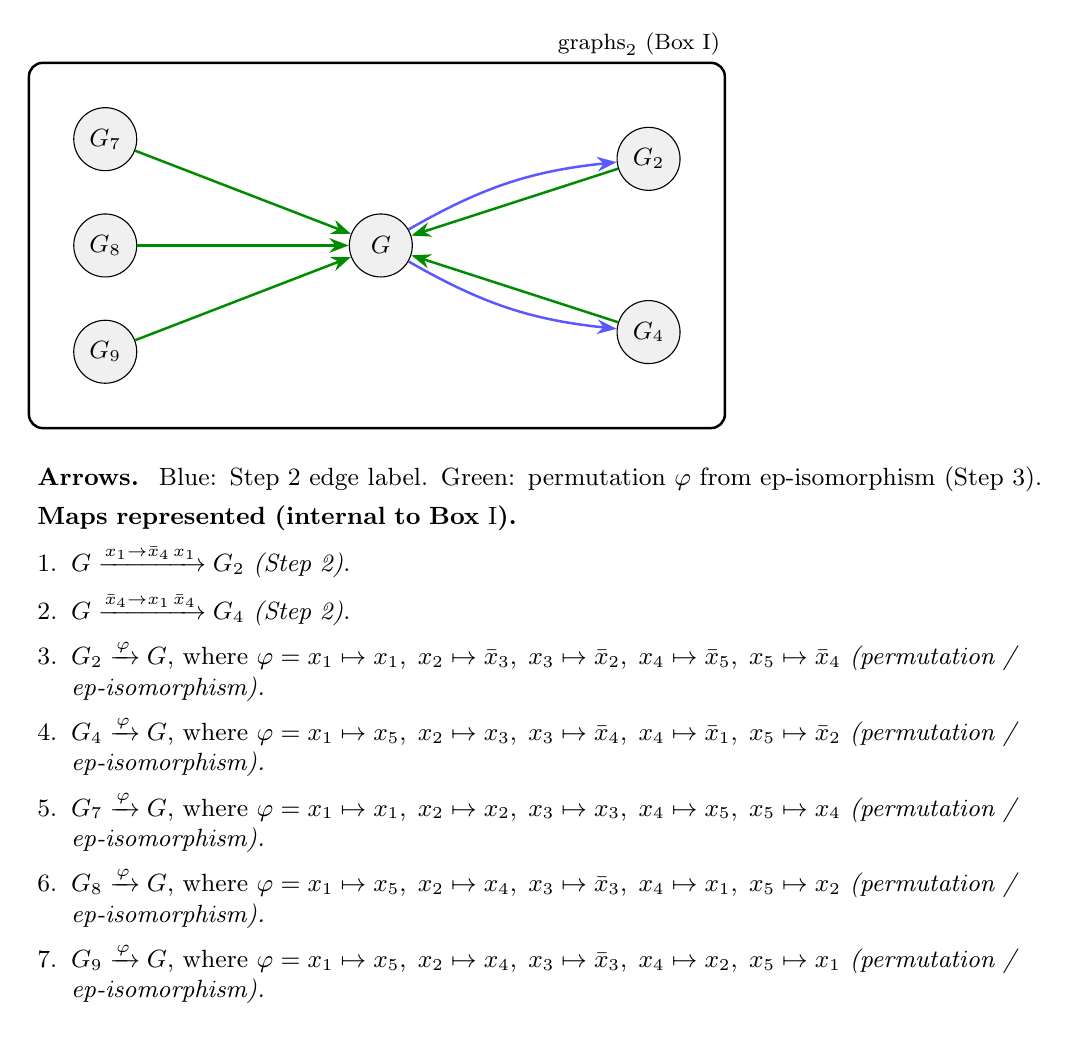
\begin{tikzpicture}[
  font=\small,
  >=Stealth,
  grnode/.style={circle, draw=black, fill=gray!12, minimum size=8mm, inner sep=1pt},
  stepmap/.style={->, draw=blue!65, line width=0.9pt},
  permmap/.style={->, draw=green!55!black, line width=0.9pt}
]
  \node[grnode] (vG) at (0.00,0.00) {$G$};
  \node[grnode] (v2) at (3.40,1.10) {$G_{2}$};
  \node[grnode] (v4) at (3.40,-1.10) {$G_{4}$};
  \node[grnode] (v7) at (-3.50,1.35) {$G_{7}$};
  \node[grnode] (v8) at (-3.50,0.00) {$G_{8}$};
  \node[grnode] (v9) at (-3.50,-1.35) {$G_{9}$};
  \draw[stepmap] (vG) to[bend left=12] (v2);
  \draw[stepmap] (vG) to[bend right=12] (v4);
  \draw[permmap] (v2) -- (vG);
  \draw[permmap] (v4) -- (vG);
  \draw[permmap] (v7) -- (vG);
  \draw[permmap] (v8) -- (vG);
  \draw[permmap] (v9) -- (vG);
  \node[draw=black, line width=0.9pt, rounded corners=5pt, inner sep=16pt, fit=(vG)(v2)(v4)(v7)(v8)(v9)] (boxframe) {};
  \node[anchor=south east, inner sep=2pt, font=\footnotesize] at (boxframe.north east) {$\mathrm{graphs}_2$ (Box $\mathrm{I}$)};
  \node[anchor=north west, align=left, text width=12.8cm] at ($(boxframe.south west)+(0,-0.35)$) {
\textbf{Arrows.}\; Blue: Step~$2$ edge label. Green: permutation $\varphi$ from ep-isomorphism (Step~$3$). \par\smallskip\textbf{Maps represented (internal to Box~$\mathrm{I}$).}
\begin{enumerate}[leftmargin=*, itemsep=2pt]
\item $G \xrightarrow{x_{1} \to \bar{x}_{4}\,x_{1}} G_{2}$ \textit{(Step~2)}.
\item $G \xrightarrow{\bar{x}_{4} \to x_{1}\,\bar{x}_{4}} G_{4}$ \textit{(Step~2)}.
\item $G_{2} \xrightarrow{\varphi} G$, where $\varphi=x_{1} \mapsto x_{1},\; x_{2} \mapsto \bar{x}_{3},\; x_{3} \mapsto \bar{x}_{2},\; x_{4} \mapsto \bar{x}_{5},\; x_{5} \mapsto \bar{x}_{4}$ \textit{(permutation / ep-isomorphism).}
\item $G_{4} \xrightarrow{\varphi} G$, where $\varphi=x_{1} \mapsto x_{5},\; x_{2} \mapsto x_{3},\; x_{3} \mapsto \bar{x}_{4},\; x_{4} \mapsto \bar{x}_{1},\; x_{5} \mapsto \bar{x}_{2}$ \textit{(permutation / ep-isomorphism).}
\item $G_{7} \xrightarrow{\varphi} G$, where $\varphi=x_{1} \mapsto x_{1},\; x_{2} \mapsto x_{2},\; x_{3} \mapsto x_{3},\; x_{4} \mapsto x_{5},\; x_{5} \mapsto x_{4}$ \textit{(permutation / ep-isomorphism).}
\item $G_{8} \xrightarrow{\varphi} G$, where $\varphi=x_{1} \mapsto x_{5},\; x_{2} \mapsto x_{4},\; x_{3} \mapsto \bar{x}_{3},\; x_{4} \mapsto x_{1},\; x_{5} \mapsto x_{2}$ \textit{(permutation / ep-isomorphism).}
\item $G_{9} \xrightarrow{\varphi} G$, where $\varphi=x_{1} \mapsto x_{5},\; x_{2} \mapsto x_{4},\; x_{3} \mapsto \bar{x}_{3},\; x_{4} \mapsto x_{2},\; x_{5} \mapsto x_{1}$ \textit{(permutation / ep-isomorphism).}
\end{enumerate}
};
\end{tikzpicture}
\end{document}
